\chapter{Aportes}

Para brindar una presentaci'on m'as clara de los aportes de esta tesis, empezaremos se\~nalando algunas caracter'isticas, falencias y limitaciones de Heterogenius en las que hemos basado cada aporte de este trabajo.

En su versi'on inicial, Heterogenius presentaba algunas limitaciones. 
A continuaci'on se detallan las que fueron tratadas en el presente trabajo.

Lo primero que se puede notar es que el nivel de granularidad en la heterogeneidad de la herramienta no es completo. 
Si bien Heterogenius permite realizar una demostraci'on en diferentes lenguajes, se limita a describir cada secuente utilizando sólo uno de ellos. 
Debido a esto se puede decir que Heterogenius en realidad permite tener demostraciones heterogeneas con secuentes homogéneos. 

Otro problema con el que nos encontramos es la incapacidad del 'arbol de an'alisis de documentar el proceso de an'alisis completo. El árbol solamente muestra las acciones y pasos que llevan al 'exito de una demostraci'on. En el momento del an'alisis cuando una rama no lleva al resultado deseado y se quieren probar otras acciones, es necesario borrar la rama que no di'o resultado. Esto lleva a que se pierdan partes del an'alisis que pueden ser 'utiles ya que documentan las acciones intentadas (que no dieron un resultado deseado) y os permite tener un historial de todo lo que se hizo en el an'alisis.

El 'arbol de an'alisis tiene solamente un tipo de ramas, que representan acciones que se tienen que llevar a cabo para que el resultado se propague al nodo raiz. Esto limita la posibilidad de realizar demostraciones alternativas y experimentar en una demostraci'on con diferentes tipos de herramientas, acciones, etc.

Debido a que las herramientas autom'aticas no siempre producen un resultado, decidimos que es necesario tambi'en documentar la aplicaci'on de las acciones a'un si no tienen un resultado definido. Todo esto aporta al objetivo general de documentar todas las acciones realizadas durante el an'alisis.

\section{Extendiendo Heterogenius con demostradores de primer orden}

Tal como se mencionó en el capítulo \ref{capitulo:TPTP-FOF}, la competencia \textit{CASC} ha adquirido una gran reputación en los últimos años.

Junto a la integraci'on de TPTP-FOF, se incorporaron los siguientes mecanismos para poder usar las herramientas correspondientes.

\begin{itemize}
\item Se permiti'o la carga de especificaciones escritas puramente en TPTP-FOF.

\item Se agreg'o una traducción $\rho$ desde el lenguaje de \textit{PDOCFA} a \textit{TPTP-FOF}. 

\item Se agregaron acciones espec'ificas que permiten invocar a las herramientas en cuesti'on.
\end{itemize}

\subsection{Traducci'on de \emph{PDOCFA} a \emph{TPTP-FOF}}

...\todomm{Esto lo escribo yo}

\todomm{Acá hay que explicar qué es un calculador de secuentes. Y se puede agregar el párrafo que está en el capítulo anterior. La explicación la podés encontrar en el paper de Manu y en su tesis.}

\subsection{Herramientas incorporadas}

Teniendo el soporte de \textit{TPTP-FOF} por parte del motor de c'alculo de secuentes de Heterogenius, integramos algunas de las herramientas mas difundidas en el 'ambito de demostradores autom'aticos de teoremas para el lenguaje \textit{TPTP-FOF}: \textit{SPASS} \cite{WDFKSW09} y \textit{E-Prover} \cite{s13} como calculadores de secuentes y \textit{Mace4} \cite{m05} y \textit{E-Prover} como buscadores de contraejemplos.

\subsubsection{SPASS}

Desde el 2000, tanto \textit{SPASS} como \textit{E-Prover} ocupan los primeros lugares en la competencia anual de demostradores de teoremas \textit{CASC} (CADE ATP System Competition).

\subsection{Modificaciones al c'alculo de Heterogenius}

Al introducir soporte para lenguajes de l'ogica de primer 'orden y herramientas autom'aticas de an'alisis de estos lenguajes, fue necesario tambi'en extender las acciones de demostraci'on de Heterogenius agregando tres reglas nuevas.

Sea $\Gamma \vdash \alpha$ el secuente que se quiere analizar, se introducen las siguientes reglas:

\begin{prooftree}
\LeftLabel{\textbf{Regla 1:}}
\AxiomC{$\top$}
\RightLabel{\qquad si vale $\Gamma \vdash^{fof} \alpha$}
\UnaryInfC{$\Gamma \vdash \alpha$}
\end{prooftree}

Esta regla indica que si se logra encontrar una demostraci'on del secuente $\Gamma \vdash \alpha$ con un demostrador autom'atico de primer orden, la rama se considera cerrada.


\begin{prooftree}
\LeftLabel{\textbf{Regla 2:}}
\AxiomC{$\bot$}
\RightLabel{\qquad si existe $\mathcal{M} \in Mod^{fof}(\Gamma$) y $\mathcal{M} \nvDash^{fof} \alpha$ }
\UnaryInfC{$\Gamma \vdash \alpha$}
\end{prooftree}

Si de lo contrario, se logra encontrar un modelo de $\Gamma$ que no satisface $\alpha$, este modelo es un contraejemplo y la rama contin'ua abierta.


\begin{prooftree}
\LeftLabel{\textbf{Regla 3:}}
\AxiomC{$\Gamma \vdash \alpha$}
\RightLabel{(si no)}
\UnaryInfC{$\Gamma \vdash \alpha$}
\end{prooftree}

Por 'ultimo, debido a que la l'ogica de primer orden no es completa y la ejecuci'on de las herramientas autom'aticas est'a limitada por un \textit{timeout}, es posible no encontrar ni una demostraci'on ni un contraejemplo. En 'este caso no se puede concluir nada y el resultado es el mismo secuente.

Con 'estas reglas se cubren todos los casos, tanto de demostraci'on como los de refutaci'on de una f'ormula de primer 'orden. Al usar alg'un demostrador autom'atico de teoremas se aplican las reglas 1 y 3. En cambio cuando se realiza una b'usqueda de contraejemplo, las reglas usadas son 2 y 3.



\section{Heterogeneidad Completa}
\label{sec:heterogeneidad-verdadera}

Para ampliar las capacidades de Heterogenius extendimos el concepto de heterogeneidad para lograr tener demostraciones completamente heterog'eneas en lugar de demostraciones heterogéneas pero con secuentes homogéneos. 

La diferencia principal radica en que, con la nueva implementaci'on, los secuentes pueden soportar f'ormulas de diferentes lenguajes. As'i un secuente puede ser de tipo homogéneo o heterogéneo. En el primer caso todas las f'ormulas del secuente usan el mismo lenguaje; en el segundo las f'ormulas son de lenguajes distintos.

La ventaja de los secuentes heterogéneos es que se pueden combinar f'ormulas (lemmas, axiomas) provenientes de distintas especificaciones escritas en lenguajes diferentes. De esta forma nos podemos abstraer del lenguaje en el que están escritas y concentrarnos en el an'alisis.

La principal limitaci'on de los secuentes heterogéneos es que las herramientas (calculadores de secuentes, buscadores de contraejemplos, demostradores autom'aticos) trabajan con secuentes escritos en un solo lenguaje, o sea secuentes homogéneos. Debido a esto se proveen nuevas operaciones para el manejo de f'ormulas dentro de un secuente.

\subsection{Operaciones para el manejo de f'ormulas}

Cada una de las siguientes operaciones puede cambiar o no la heterogeneidad de un secuente.  Dependiendo de los lenguajes de las f'ormulas del resultado, el secuente puede pasar a ser heterogéneo, homogéneo o mantener su tipo. Las nuevas operaciones que permiten disponer de un mayor control sobre la heterogeneidad de los secuentes son:

\begin{itemize}
\item Proyecci'on
\item Introducci'on de antecedentes desde una fuente externa
\item Traducci'on
\end{itemize}

\subsubsection{Proyecci'on}

'Esta operaci'on  permite seleccionar un subconjunto de las f'ormulas que se quiere proyectar sobre el secuente actual y el nuevo secuente se forma a partir de las f'ormulas seleccionadas:

%$$ \alpha_1,\ldots,\alpha_n \vdash \alpha_{n+1},\ldots,\alpha_m $$
%\begin{prooftree}
%\AxiomC{$\alpha_1$,$\ldots$,$\alpha_n$}
%\UnaryInfC{$\alpha_{n+1}$,$\ldots$,$\alpha_m$}
%\end{prooftree}

\begin{prooftree}
\AxiomC{$\{\alpha_{i\in [1,n]\cap\mathcal{C}} \} \vdash \{\alpha_{j\in [n+1, m]\cap\mathcal{C}}\}$}
\RightLabel{Regla de proyecci'on}
\UnaryInfC{$ \alpha_1,\ldots,\alpha_n \vdash \alpha_{n+1},\ldots,\alpha_m $}
\end{prooftree}

con $\mathcal{C} \subseteq \{1 \ldots m\}$, un subconjunto de los 'indices de las f'ormulas que se quieren proyectar.

%\begin{prooftree}
%\AxiomC{$\alpha_i$ con $i=1 \ldots n$ y $i \in \mathcal{C}$}
%\UnaryInfC{$\alpha_j$ con $j=n+1 \ldots m$ y $j \in \mathcal{C}$}
%\end{prooftree}
%$$\{\alpha_i \} \vdash \{\alpha_j\} \mbox{ con }i\in [1,n]\cap\mathcal{C} \mbox{ y } j\in [n+1, m]\cap\mathcal{C}$$
%\vspace{1em}

Si se aplica una operaci'on de proyecci'on a un secuente homog'eneo el resultado siempre ser'a homog'eneo, pero si se empieza con un secuente heterogeneo el resultado puede ser un secuente homog'eneo, si se proyectan f'ormulas de un mismo lenguaje o un secuente heterog'eneo si la proyecci'on incluye f'ormulas de lenguajes diferentes.

A modo de ejemplo, en la Fig.~\ref{seq selection} se muestra el cuadro de di'alogo mediante el cual el usuario puede seleccionar las f'ormulas que se quiere proyectar en el nuevo secuente. Notar que el secuente presentado es heterog'eneo y contiene formulas tanto en \textit{Alloy} como en \textit{TPTP-FOF}.

\begin{figure}[]
	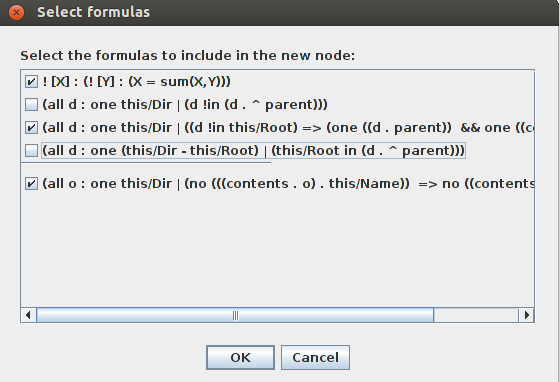
\includegraphics[width=200px]{img/select.png}
	\centering
	\caption{(Cuadro de di'alogo de proyecci'on de f'ormulas)}
        \label{seq selection}
\end{figure}

\subsubsection{Introducci'on de f'ormulas desde una fuente externa}

Esta operaci'on es una generalizaci'on de la regla de corte, que permite cargar f'ormulas desde un archivo de especificaci'on, ya sea escrito en el lenguaje \textit{Alloy} o en \textit{TPTP-FOF}. Al seleccionar las f'ormulas nuevas, se crean dos nodos nuevos que se agregan como hijos del nodo actual. Las f'ormulas a su vez se introducen como hip'otesis en uno de los secuentes y como tesis en el otro.

La operaci'on se puede ejecutar a trav'ez del men'u contextual que se muestra en la Fig. \ref{add antecedents 1}.


\begin{prooftree}
\AxiomC{$ \Gamma,\beta_1,\ldots, \beta_k \vdash \Delta $}
\AxiomC{$ \Gamma\vdash \beta_1,\ldots, \beta_k , \Delta $}
\RightLabel{(Regla de introducci'on de f'ormulas nuevas)}
\BinaryInfC{$ \Gamma \vdash \Delta $}
\end{prooftree}

con $\{\beta_1 \ldots \beta_k\}$ un conjunto de f'ormulas nuevas a introducir.

%\begin{prooftree}
%\AxiomC{$\alpha_1$,$\ldots$,$\alpha_n$}
%\UnaryInfC{$\alpha_{n+1}$,$\ldots$,$\alpha_m$}
%\end{prooftree}
%$$ \alpha_1,\ldots,\alpha_n \vdash \alpha_{n+1},\ldots,\alpha_m $$
%y un conjunto de f'ormulas nuevas $\{\beta_1 \ldots \beta_k\}$. El nuevo secuente es:
%\begin{prooftree}
%\AxiomC{$\alpha_1$,$\ldots$,$\alpha_n,\beta_1,\ldots, \beta_k$}
%\UnaryInfC{$\alpha_{n+1}$,$\ldots$,$\alpha_m$}
%\end{prooftree}
%$$ \alpha_1,\ldots,\alpha_n,\beta_1,\ldots, \beta_k \vdash \alpha_{n+1},\ldots,\alpha_m $$

'Esta operaci'on puede puede conservar o cambiar tanto la homogeneidad como la heterogeneidad del secuente inicial.

\begin{figure}
\centering
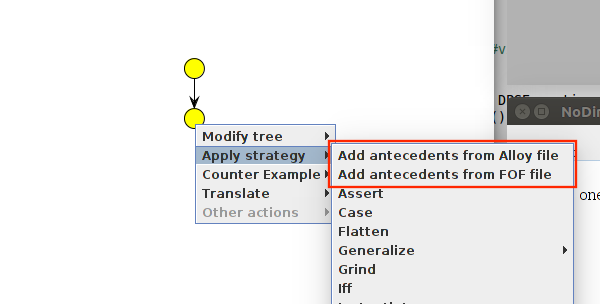
\includegraphics[width=5cm]{img/add_antecedents_1.png}	
\caption{Men'u contextual para seleccionar la fuente de las f'ormulas a introducir.}
\label{add antecedents 1}
\end{figure}


\subsubsection{Traducci'on}

Se extendi'o el concepto de traducciones para que se puedan traducir f'ormulas por separado, en lugar de traducir un secuente completo como en la versi'on anterior.
El secuente resultante contendr'a las f'ormulas del secuente analizado en el lenguaje seleccionado.

\begin{prooftree}
\AxiomC{$ \rho_{\mathcal{T}(\alpha_1)}(\alpha_1) ,\ldots, \rho_{\mathcal{T}(\alpha_n)}(\alpha_n) \vdash \rho_{\mathcal{T}(\alpha_{n+1})}(\alpha_{n+1}) ,\ldots,\rho_{\mathcal{T}(\alpha_m)}(\alpha_m) $}
\RightLabel{(Regla de traducci'on)}
\UnaryInfC{$ \alpha_1,\ldots,\alpha_n \vdash \alpha_{n+1},\ldots,\alpha_m $}
\end{prooftree}

donde $\rho_l$ es la funci'on de traducci'on al lenguaje $L$ y $\mathcal{T}:Formula\rightarrow Lenguaje$ que indica el lenguaje seleccionado para cada f'ormula del secuente original.

%$$ S: \alpha_1,\ldots,\alpha_n \vdash \alpha_{n+1},\ldots,\alpha_m $$
%\begin{prooftree}
%\AxiomC{$\alpha_1$,$\ldots$,$\alpha_n$}
%\UnaryInfC{$\alpha_{n+1}$,$\ldots$,$\alpha_m$}
%\end{prooftree}
%y una función  $\mathcal{T}:Formula\rightarrow Lenguaje$ que indica el lenguaje seleccionado para cada f'ormula del secuente $S$, el secuente resultante es:
%$$ S': \beta_1,\ldots,\beta_n \vdash \beta_{n+1},\ldots,\beta_m $$
%\begin{prooftree}
%\AxiomC{$\beta_1$,$\ldots$,$\beta_n$}
%\UnaryInfC{$\beta_{n+1}$,$\ldots$,$\beta_m$}
%\end{prooftree}


En la Fig. \ref{GUI form translation} se puede ver un cuadro de di'alogo donde el usuario puede seleccionar, para cada f'ormula, el lenguaje al que se quiere traducir.

\begin{figure}[]
	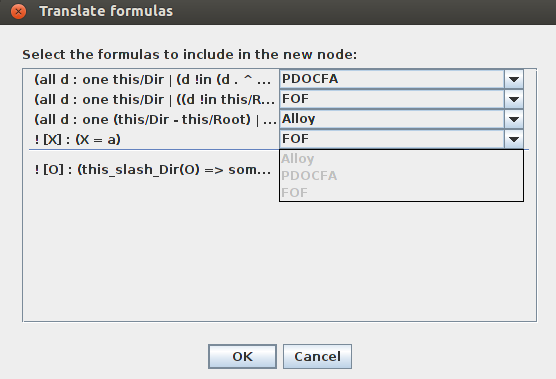
\includegraphics[width=200px]{img/translate.png}
	\centering
	\caption{Cuadro de di'alogo para la traducci'on de f'ormulas en un secuente.} \label{GUI form translation}
\end{figure}



\section{Rediseño del 'Arbol de An'alisis}

Para solucionar las limitaciones presentadas nos propusimos rediseñar el 'arbol de an'alisis.
El primer cambio que realizamos es la implementaci'on de \emph{heterogeneidad completa}.
Para lograr esto permitimos que también los secuentes sean heterogéneos, es decir, que puedan contener f'ormulas escritas en distintos lenguajes. De esta manera se consigue realizar las demostraciones con mayor flexibilidad y poder utilizar el lenguaje m'as apropiado para describir la propiedad que cada f'ormula enuncia.
La implementaci'on y los fundamentos te'oricos se explican con mayor detalle en la secci'on \hyperref[sec:heterogeneidad-verdadera]{\ref*{sec:heterogeneidad-verdadera} }.

En el 'arbol de an'alisis este cambio se refleja en la visualizaci'on de los nodos. Los nodos con secuentes heterogéneos se marcan con una \textit{H} mientras los nodos homogéneos no llevan ninguna marca.

\begin{figure}[tbh]
	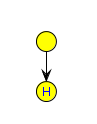
\includegraphics[width=50px]{img/hetero_homo.png}
	\centering
	\caption{El nodo con H contiene un secuente heterog'eneo. El otro nodo es homog'eneo.}
\end{figure}


\subsection{Ramas alternativas}

Para permitir documentar todas las acciones aplicadas as'i como la creaci'on de caminos de an'alisis alternativos introdujimos la noci'on de \textit{ramificaci'on alternativa}.
Las ramas alternativas representan la existencia de m'ultiples caminos en los que se subdivide el an'alisis para lograr un resultado. En la interfaz de usuario de Heterogenius este tipo de ramas se representa con lineas punteadas y su significado sem'antico es el de una disyunci'on. Se corresponde con un camino alternativo en una demostraci'on.

\begin{figure}[htb]
	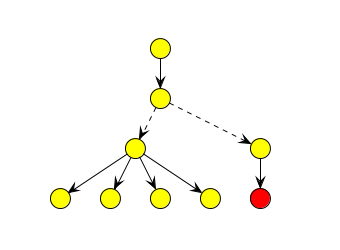
\includegraphics[width=180px]{img/ramas_alternativas_2.png}
	\centering
	\caption{La segunda rama alternativa presenta un contraejemplo. esto indica que existe un contraejemplo para el nodo del cual salen las ramas alternativas.}
        \label{alter1}
\end{figure}

Un nodo con hijos conectados por ramas alternativas se entiende que vale si \textit{\textbf{alguna}} de las ramas valen. Esto es diferente de la ramificaci'on normal (lineas continuas) que indica que el nodo padre vale si todos sus hijos valen.

Al aplicar una ramificaci'on alternativa a un nodo del 'arbol de an'alisis, el nodo es copiado y agregado como sus propios hijos. Esto nos permite trabajar sobre las copias del nodo original. Cuando es necesario tambi'en se puede agregar ramas alternativas durante un an'alisis.
 
La principal ventaja de usar caminos alternativos es la de poder documentar todo el an'alisis que se realiz'o y las decisiones tomadas, incluso las decisiones que no llevaron al cumplimiento del objetivo. Por otro lado tambi'en nos permite experimentar con diferentes formas de probar lo mismo.
En las Fig.~\ref{alter1} y \ref{alter2} se muestran ejemplos de estos usos.

\begin{figure}[bth]
	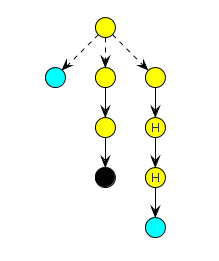
\includegraphics[width=100px]{img/ramas_alternativas.png}
	\centering
	\caption{Tres ramas alternativas: la primera y la 'ultima indican que no se encontr'o ning'un contraejemplo. La segunda rama muestra que se pudo demostrar que el secuente vale, por lo cu'al el secuente del nodo raiz tambi'en vale.}
        \label{alter2}
\end{figure}



\subsection{Nueva Clasificaci'on de Acciones}

Como se ha mencionado, el elemento principal del proceso de demostración en Heterogenius es el 'arbol de an'alisis. All'i es donde se realizan todas las acciones y es donde se refleja el camino tomado para lograr una demostraci'on exitosa. Cada nodo del 'arbol representa un secuente en alg'un lenguaje soportado por Heterogenius. Las aristas se corresponden con las acciones aplicadas a cada secuente. Dependiendo del lenguaje en el que est'e el secuente se habilitan distintas acciones, pero en general se las puede dividir en tres categor'ias:

\begin{description}
\label{clasificacion}
\item[\textbf{reglas del c'alculo de secuentes}:] son acciones que transforman un secuente en otro. Algunas pueden producir múltiples secuentes (por ejemplo la acci'on \emph{Case}) creando varias ramas que tienen que ser demostradas para lograr un resultado en el nodo raiz.

\item[\textbf{traducciones}:] traducen un secuente de un lenguaje a otro. Dependiendo de la expresividad del lenguaje esta traducci'on puede preservar completamente la semántica o sólo parcialmente.

\item[\textbf{búsquedas de contraejemplos}:] implican el uso de herramientas externas para buscar contraejemplos para intentar validar el secuente donde se aplica la acci'on. 
Dependiendo del lenguaje del secuente y del poder de la herramienta seleccionada para realizar la búsqueda, estos procesos pueden verse como análisis parciales ya que podría ser imposible agotar todo el espacio de búsqueda. En tales contextos, una búsqueda infructuosa no brinda mayor información. Por el contrario, la existencia de un contraejemplo es prueba suficiente para saber que la rama en cuestión no podrá ser cerrada.
\end{description}

Si bien esta clasificaci'on serv'ia en la versi'on anterior, debi'o ser modificada para adaptarse a la nueva funcionalidad incluida durante el desarrollo de este trabajo y permitir una mayor flexibilidad a la hora de agregar otras herramientas en el futuro.
La nueva clasificaci'on propuesta se muestra a continuaci'on.

\begin{description}
\item[\textbf{Acciones de c'alculo de secuentes}:] esta categor'ia es ls misma que en la versi'on anterior. Comprende las acciones que permiten avanzar en el an'alisis aplicando reglas del c'alculo de secuentes.

\item[\textbf{Acciones de herramientas estructurales}:] son acciones que trabajan directamente sobre la estructura del 'arbol de an'alisis. Los traductores-$\rho$ forman parte de 'este grupo, asi como las nuevas acciones introducidas: \textit{traducci'on-$\rho$ de f'ormulas} y \textit{proyecci'on de f'ormulas}.

\item[\textbf{Acciones de herramientas automáticas}:] este grupo representa a las acciones para las que se usan herramientas autom'aticas como lo son los demostradores autom'aticos de teoremas y los buscadores de contraejemplos.
\end{description}

Esta clasificaci'on se reflej'o en la arquitectura de Heterogenius y permitir'a guiar las futuras extensiones y funcionalidades adicionales que se deseen implementar.


\section{Detalles de Implementaci'on}

En 'esta secci'on se explicar'an algunas de las dificultades y detalles de las decisiones tomadas al implementar los nuevos conceptos en \textit{Heterogenius}. En particular vamos a explicar la extensi'on de las traducciones $\rho$, la integraci'on del lenguaje \textit{TPTP-FOF} e implementaci'on de buscadores de contraejemplo y demostradores usando las herramientas autom'aticas que trabajan con el lenguaje \textit{TPTP-FOF}.

\subsection{Extensi'on de las traducciones Rho}

\todomm{El punto fuerte de tu trabajo fue la implementación de estos conceptos, así que tenemos que explicar bien esto como para que los jurados lo entiendan así. En principio, deberías explicar un poco cómo estaba diseñado Heterogenius, para que se entienda la magnitud del cambio que realizaste}

Debido a los cambios introducidos fue necesario \textit{refactorizar} el diseño de la infraestructura de las traducciones $\rho$. Lo primero que se hizo fue agregar un \textit{TranslationsManager}, un objeto encargado de manejar todas las traducciones soportadas por el sistema. 

Por otro lado los traductores (subclases de \textit{Translator}) deben implementar los tres m'etodos  abstractos definidos en la clase padre. Cada uno de 'estos m'etodos permite un control m'as fino de las traducciones al separar el secuente en sus partes, que son: una referencia de skolemizac'ion, una especificaci'on y la f'ormula analizada.

\begin{figure}[H]
	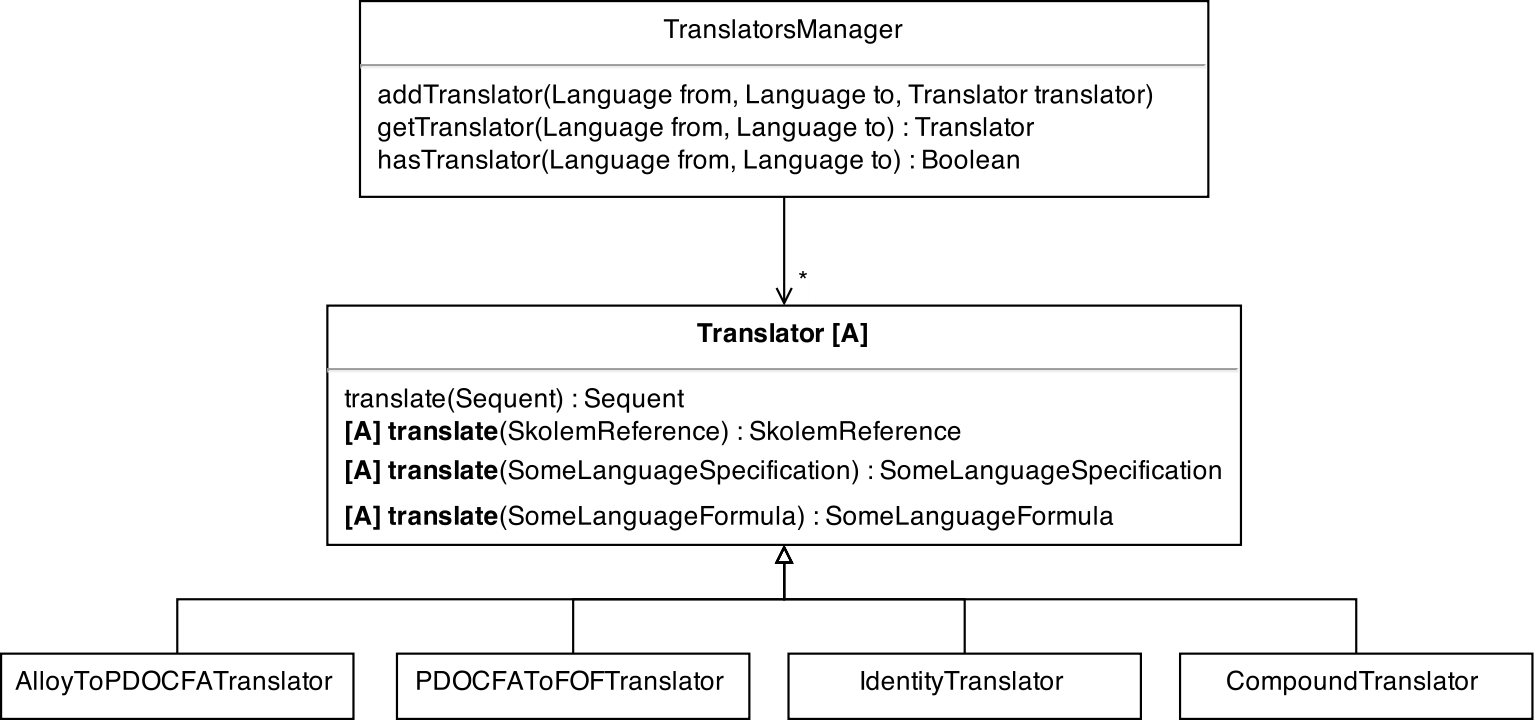
\includegraphics[width=400px, angle=90]{img/arq_traductores.png}
\end{figure}

Se proveen los traductores de \textit{Alloy} a \textit{PDOCFA}, de \textit{PDOCFA} a \textit{TPTP-FOF} asi como el \textit{CompoundTranslator} que permite componer los traductores para lograr traducciones transitivas, por ejemplo de \textit{Alloy} a \textit{TPTP-FOF}.


\subsection{Demostradores de teoremas}

\subsubsection{Preparaci'on del secuente}

El formato \textit{TPTP-FOF} que usan las herramientas autom'aticas agregadas es una lista de f'ormulas escritas en el lenguaje \textit{TPTP-FOF}. Cada una de 'estas f'ormulas debe tener un tipo que puede ser: \textit{axiom} o \textit{conjecture} (existen m'as tipos pero son irrelevantes para nuestro caso).

Para convertir el secuente analizado al formato \textit{TPTP-FOF} se agregan todas las f'ormulas del antecedente con el tipo \textit{axiom} y las f'ormulas del consecuente con el tipo \textit{conjecture}. 

Al ejecutar un demostrador autom'atico con la entrada preparada de este modo, se va a tratar de probar las f'ormulas del consecuente usando que las f'ormulas del antecedente son verdaderas.


\subsubsection{Integraci'on con Heterogenius}

Para integrar las herramientas autom'aticas, tanto los demostradores de teoremas como los buscadores de contraejemplos fue necesario \textit{refactorizar} y extender el diseño de algunas partes de la arquitectura de Heterogenius. Algunos de los objetivos y criterios que se usaron durante el rediseño fueron lograr abstraer las herramientas usadas y hacer un diseño lo suficientemente extensible y abierto para la integraci'on con nuevas herramientas en el futuro.

\begin{figure}[H]
	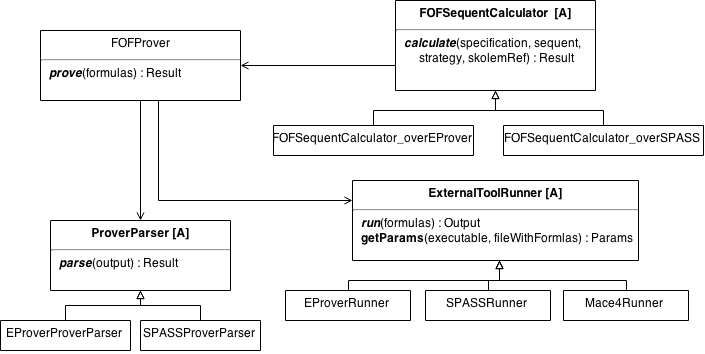
\includegraphics[width=450px, angle=90]{img/arq_prover.png}
	\centering
	\caption{Demostradores autom'aticos usados como calculadores de secuentes.}
\end{figure}

\todomm{Mencionar en la explicación qué roles desempeñan cada una de las entidades mencionadas. Además indicar explícitamente cuáles debieron ser modificadas y cuáles agregadas en la nueva versión.
Para explicar esto podés indicar los pasos que se deberían seguir para incorporar un demostrador nuevo (como lo que está en estos dos párrafos, pero explicado con más detalle).
Y explicar cómo fueron implementados esos pasos para incluir alguno de los demostradores que agregaste.}

Un calculador de secuentes basado en un demostrador autom'atico del lenguaje \textit{TPTP-FOF} se crea subclasificando la clase abstracta \textbf{FOFSequentCalculator}. La nueva clase va a contener un objeto \textit{FOFProver} compuesto con los objetos de las subclases de \textbf{ProverParser} y de \textbf{ExternalToolRunner} correspondientes.

Para agregar una herramienta nueva primero se debe subclasificar la clase abstracta \textbf{ExternalToolRunner}. Esta clase abstrae las particularidades de ejecuci'on de la herramienta especificando los parametros necesarios. Luego se extiende la clase \textbf{ProverParser} que se encarga de procesar el texto correspondiente a la salida de la herramienta. 



\subsection{B'usqueda de contraejemplos}

\subsubsection{Preparaci'on del secuente}

Tanto \textit{Mace4} como \textit{E-Prover} se usan para buscar contraejemplos de los secuentes \textit{TPTP-FOF}. Como las dos herramientas son buscadores de modelos, para preparar el secuente lo que se hace es armar una lista de f'ormulas de tipo \textit{axiom} a partir de las f'ormulas del antecedente y del consecuente del secuente analizado.

Cuando todas las f'ormulas que se envian como entrada a los buscadores de modelos son de tipo \textit{axiom}. Las herramientas tratan de buscar un modelo para el conjunto de los axiomas recibidos.

Lo que se quiere lograr es encontrar un contraejemplo, entonces se hace necesario negar el secuente y buscar un modelo para la negaci'on.

Sea $\{\alpha_1 \dots \alpha_n\} \vdash \{\beta_1 \dots \beta_m\}$ el secuente bajo an'alisis.
La negaci'on se puede escribir como:

\begin{equation}
\bigwedge\limits_{i=1}^n{\alpha_i} \wedge \bigwedge\limits_{j=1}^m{\neg \beta_{j}}
\end{equation}

Con lo cual para armar la lista de f'ormulas de entrada, para cada $\alpha_{i}$ del antecedente se agrega $\alpha_{i}$ como axioma y para cada $\beta_{i}$ del consecuente se agrega $\neg \beta_{i}$ tambi'en como axioma.

Encontrar un modelo para una especificaci'on armada de 'este modo implica la existencia de un contraejemplo para el secuente procesado.


\subsubsection{Integraci'on con Heterogenius}

Tambi'en como en el caso de los demostradores autom'aticos fue necesario \textit{refactorizar} el diseño de los buscadores de contraejemplos para permitir una mayor flexibilidad a la hora de agregar nuevas herramientas con soporte de \textit{TPTP-FOF}.

\begin{figure}[H]
	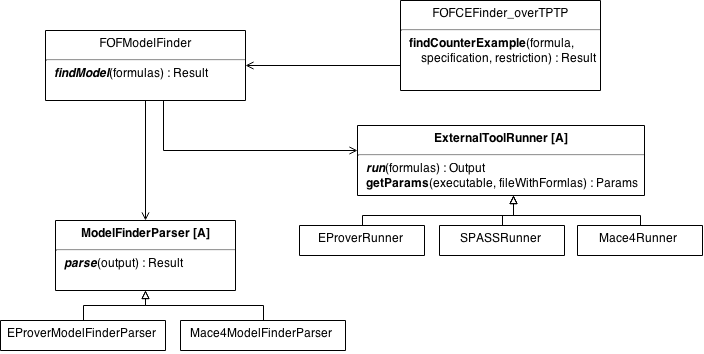
\includegraphics[width=450px, angle=90]{img/arq_ce.png}
	\centering
	\caption{Buscadores de contraejemplos.}
\end{figure}

\todomm{Ídem anterior (a menos que queden demasiado parecidos).}
El diseño de los buscadores de contraejemplos basados en \textit{TPTP-FOF} es an'alogo a los calculadores de secuentes. Se usa la misma clase \textbf{ExternalToolRunner} que en el caso anterior para la abstracci'on de la ejecuci'on de la herramienta en s'i. Pero en lugar de subclasificar \textbf{ProverParser} se subclasifica la clase abstracta \textbf{ModelFinderParser} que tiene un comportamiento an'alogo.

%á
